\documentclass[11pt,a4paper]{article}

\usepackage[utf8]{inputenc}
\usepackage{geometry}
\geometry{top=2.5cm, bottom=2.5cm, left=2.5cm, right=2.5cm}
\usepackage{graphicx}
\usepackage{booktabs}
\usepackage{amsmath,amssymb}
\usepackage{hyperref}
\usepackage{xcolor}
\usepackage{float}
\usepackage{caption}
\usepackage{subcaption}
\usepackage{microtype}
\usepackage{listings}
\usepackage{adjustbox}
\usepackage{makecell}

\definecolor{codegray}{rgb}{0.5,0.5,0.5}
\definecolor{backcolour}{rgb}{0.96,0.96,0.96}
\lstset{
    backgroundcolor=\color{backcolour},
    basicstyle=\ttfamily\small,
    breaklines=true,
    captionpos=b,
    keepspaces=true,
    numbers=left,
    numberstyle=\tiny\color{codegray},
    showspaces=false,
    showstringspaces=false,
    showtabs=false,
    tabsize=2
}

\hypersetup{
    colorlinks=true,
    linkcolor=blue!70!black,
    citecolor=blue!70!black,
    urlcolor=blue!70!black
}

\title{\textbf{Comprehensive Phase 1 Technical Report:\\ReXGroundingCT 3D Data Profiling, Spatial Priors, and Prompt Syntax Analysis}}

\author{\textbf{ReXGroundingCT Challenge Research Team}\\
\small MICCAI 2026 Challenge Benchmark Investigation}

\date{July 28, 2026}

\begin{document}

\maketitle

\begin{abstract}
This technical report synthesizes the quantitative results of the consolidated Phase 1 profiling suite (\texttt{exp\_001} through \texttt{exp\_005}) conducted for the ReXGroundingCT MICCAI 2026 Challenge~\cite{baharoon2025rexgroundingct}. Analyzing 3,192 3D thoracic CT scan entries (representing 3,078 physical NIfTI volumes derived from the CT-RATE repository~\cite{hamamci2024ctrate}) and 8,650 radiology report finding prompts across 14 official finding categories, we investigate annotation disparity between training and validation splits, patient hierarchy and cross-split leakage, free-text prompt syntax shift, canonical RAS 3D spatial probability density distributions, physical Hounsfield Unit (HU) radiodensity attenuation bounds, and 3D morphological topology across 27,138 discrete connected components. We establish calibrated actionable modeling and post-processing directives to guide downstream zero-shot baseline evaluation with VoxTell~\cite{luo2025voxtell} and model fine-tuning.
\end{abstract}

\tableofcontents
\newpage

\section{Executive Summary \& Research Context}

\subsection{Benchmark Challenge Overview \& Dataset Hierarchy}
The ReXGroundingCT Challenge @ MICCAI 2026 evaluates automated multi-modal 3D grounding models tasked with segmenting anatomical pathologies in 3D thoracic Computed Tomography (CT) scans (derived from the CT-RATE repository~\cite{hamamci2024ctrate}) from free-text radiology finding descriptions. 

To eliminate confusion across dataset metrics, we formally define the 4-tier dataset indexing structure:
\begin{itemize}
    \item \textbf{Tier 1: Physical NIfTI Scans (3,078 volumes)}: The underlying physical ground-truth image repository containing 2,578 Training scans, 200 Validation scans, and 300 Test scans acquired from distinct CT scan acquisition sessions.
    \item \textbf{Tier 2: Dataset Record Entries (3,192 entries)}: The primary indexing entries stored in \texttt{dataset.json} (comprising 2,992 Training entries and 200 Validation entries). The total indexed record entries (3,192) exceed physical scan acquisitions (3,078) because multiple reconstruction series (e.g., soft-tissue vs.\ high-resolution lung kernels, or thin vs.\ thick slice reconstructions \texttt{\_1.nii.gz}, \texttt{\_2.nii.gz}) derived from a single physical CT examination are indexed as separate entries in \texttt{dataset.json}. Test split entries (300 physical scans) are withheld from \texttt{dataset.json} pending official challenge submission.
    \item \textbf{Tier 3: Target Findings (8,650 target findings total, 8,068 in indexed Train+Val)}: Discrete 3D target segmentation masks (7,687 in Train, 381 in Val, 582 in Test). As specified in the official ReXGroundingCT paper~\cite{baharoon2025rexgroundingct}, findings were extracted from radiology reports using GPT-4. Under the training set's \textit{Entity Protocol}, annotators were instructed to segment at most three representative instances per finding ($\le 3$ instances/finding, mean $1.95$) to manage annotation workload. Conversely, the Validation split features unconstrained exhaustive annotation of all visible instances (mean $3.71$, reaching up to 36 instances). Test split ground-truth instance masks are withheld from challenge participants for evaluation integrity, resulting in placeholder values ($\text{mean} = 1.000 \pm 0.000$, $\text{max} = 1$) in raw benchmark metadata.
    \item \textbf{Tier 4: Radiology Report Prompts (8,650 prompts)}: Free-text sentence queries extracted across all findings (7,687 in Train, 381 in Val, 582 in Test). Each radiology report prompt is paired 1-to-1 with a target finding mask, averaging $2.57$ findings/prompts per CT scan record in Train ($\frac{7,687}{2,992} = 2.5692$) and $2.53$ overall in Train+Val ($\frac{8,068}{3,192} = 2.5276$). Across the benchmark, 7,040 prompts ($81.4\%$) are unique verbatim text strings, while 1,610 ($18.6\%$) are exact duplicate sentences resulting from standardized clinical template descriptions and multi-kernel CT reconstruction series.
\end{itemize}

\subsection{Dataset Metadata Indexing Structure (\texttt{dataset.json})}
Master dataset metadata is organized in \texttt{dataset.json} as a dictionary indexing the Training (\texttt{"train"}, 2,992 records) and Validation (\texttt{"val"}, 200 records) splits, totaling 3,192 records. Test split entries are withheld pending submission. Listing~\ref{lst:dataset_sample} illustrates a representative entry (\texttt{train\_1935\_a\_1.nii.gz}) demonstrating multi-finding annotations:

\begin{lstlisting}[language=json,caption={Representative \texttt{dataset.json} record entry (\texttt{train\_1935\_a\_1.nii.gz}) illustrating finding descriptions, categories, component counts, pixel volumes, and spatial matrix shapes.},label={lst:dataset_sample}]
{
  "name": "train_1935_a_1.nii.gz",
  "findings": {
    "0": "Segmental and subsegmental peribronchial thickening with prominent luminal narrowing in both lungs",
    "1": "Mosaic attenuation pattern in both lungs",
    "2": "Reticulonodular density increases in both lung apices",
    "3": "Paraseptal emphysema in both lung apices",
    "4": "Several subcentimeter nonspecific pulmonary nodules in both lungs"
  },
  "entity_counts": {
    "0": 2,
    "1": 3,
    "2": 2,
    "3": 3,
    "4": 3
  },
  "shape": [512, 512, 264],
  "pixels": {
    "0": 101934,
    "1": 315619,
    "2": 10405,
    "3": 7065,
    "4": 772
  },
  "categories": {
    "0": "1a",
    "1": "1f",
    "2": "1d",
    "3": "1c",
    "4": "2d"
  }
}
\end{lstlisting}

\bigskip

\section{Phase 1 Consolidated 5-Experiment Mapping Index}

To establish clean modular boundaries and maintain reproducible computation, the Phase 1 profiling suite was consolidated into five standardized experiments, each pairing a computational Python script, a structured output JSON artifact, and a documentation report:

\begin{enumerate}
    \item \textbf{Experiment 001 (\texttt{exp\_001\_dataset\_disparity\_leakage})}: Dataset composition, sparse Train vs.\ exhaustive Val mask disparity, positive-unlabeled (PU) loss justification, 3-tier patient hierarchy, and cross-split leakage audit.
    \item \textbf{Experiment 002 (\texttt{exp\_002\_nlp\_prompt\_syntax})}: Free-text NLP prompt syntax shift (Cases 1--50 vs.\ 51--200), BPE subword tokenization dynamics (+34.7\% expansion, 1.347x ratio), spatial preposition locators (64.39\%), and diagnostic hedging pruning (0.38\%).
    \item \textbf{Experiment 003 (\texttt{exp\_003\_spatial\_density\_priors})}: 3D RAS spatial centroids $(RL, AP, IS)$, 4-tier spatial density prior taxonomy (Apical, Basal, Hilar, Isotropic), cosine similarity $S_{cos}$, centroid shift $\Delta d$, and 4-panel population density prior figure across all 14 categories ($128 \times 128 \times 128$ grid).
    \item \textbf{Experiment 004 (\texttt{exp\_004\_hu\_radiodensity})}: Hounsfield Unit (HU) attenuation profiling inside mask regions vs.\ surrounding parenchyma across all 14 categories, contrast deltas ($\Delta \text{HU}$), and category intensity windowing bounds \texttt{[min\_HU, max\_HU]}.
    \item \textbf{Experiment 005 (\texttt{exp\_005\_morphology\_noise\_pruning})}: 3D connected-component morphology across 27,138 blobs, sphericity index ($S$), surface area-to-volume ($SA/V$) ratios, volume quantiles, and recommended noise pruning thresholds (\texttt{recommended\_min\_size\_voxels}).
\end{enumerate}

\bigskip

\section{Exp 001: Statistical Mask Analysis, Entity Counts \& Patient Leakage}

\subsection{Split Composition \& Annotation Disparity}
A key empirical finding of Experiment 001 is the quantitative disparity between the partially annotated Training split and the exhaustively annotated Validation split, summarized in Table~\ref{tab:split_summary}.

\begin{table}[H]
\centering
\caption{Dataset split overview highlighting the annotation disparity between Train (Entity Protocol $\le 3$), Val (Exhaustive), and Test (Withheld ground truth).}
\label{tab:split_summary}
\begin{adjustbox}{max width=\linewidth}
\small
\setlength{\tabcolsep}{6pt}
\begin{tabular}{lcccccc}
\toprule
\textbf{Split} & \makecell{\textbf{Records /}\\\textbf{Physical Scans}} & \textbf{Findings} & \makecell{\textbf{Findings}\\\textbf{/Record}} & \makecell{\textbf{Mean Inst}\\\textbf{/Find}} & \textbf{Std Inst} & \textbf{Max Inst} \\
\midrule
Train & 2,992 (2,578) & 7,687 & 2.57 & 1.948 & $\pm 0.962$ & 11 \\
Val   & 200 (200)     & 381   & 1.91 & 3.714 & $\pm 4.441$ & 36 \\
Test  & 300 (300)$^*$ & 582   & 1.94 & 1.000$^\dagger$ & $\pm 0.000$ & 1 \\
\bottomrule
\end{tabular}
\end{adjustbox}
\vspace{2mm}
\raggedright \footnotesize $^*$Test split records are withheld from \texttt{dataset.json} during Phase 1. $^\dagger$Test split instance masks are withheld for official benchmark evaluation, displaying single placeholder instance metadata ($1.000 \pm 0.000$).
\end{table}

Under the Training set's \textit{Entity Protocol}, annotators segment representative instances per finding query ($\le 3$ annotated instances in typical findings, mean $1.948 \pm 0.962$, peaking at 11 in rare multi-focal entries). Conversely, the Validation split features unconstrained exhaustive annotation ($\text{Max}=36$, $\mu=3.714 \pm 4.441$). Standard binary cross-entropy (BCE) or Dice losses treat unannotated true-positive voxels as negative background, introducing instance suppression bias. This empirically justifies Positive-Unlabeled (PU) loss formulations (such as PU SPOCO) during fine-tuning.

\begin{figure}[H]
\centering
\begin{subfigure}[b]{0.48\textwidth}
    \centering
    
\includegraphics[width=\textwidth]{fig/exp001_category_frequency_breakdown.png}
    \caption{Category frequency distribution across splits.}
\end{subfigure}
\hfill
\begin{subfigure}[b]{0.48\textwidth}
    \centering
    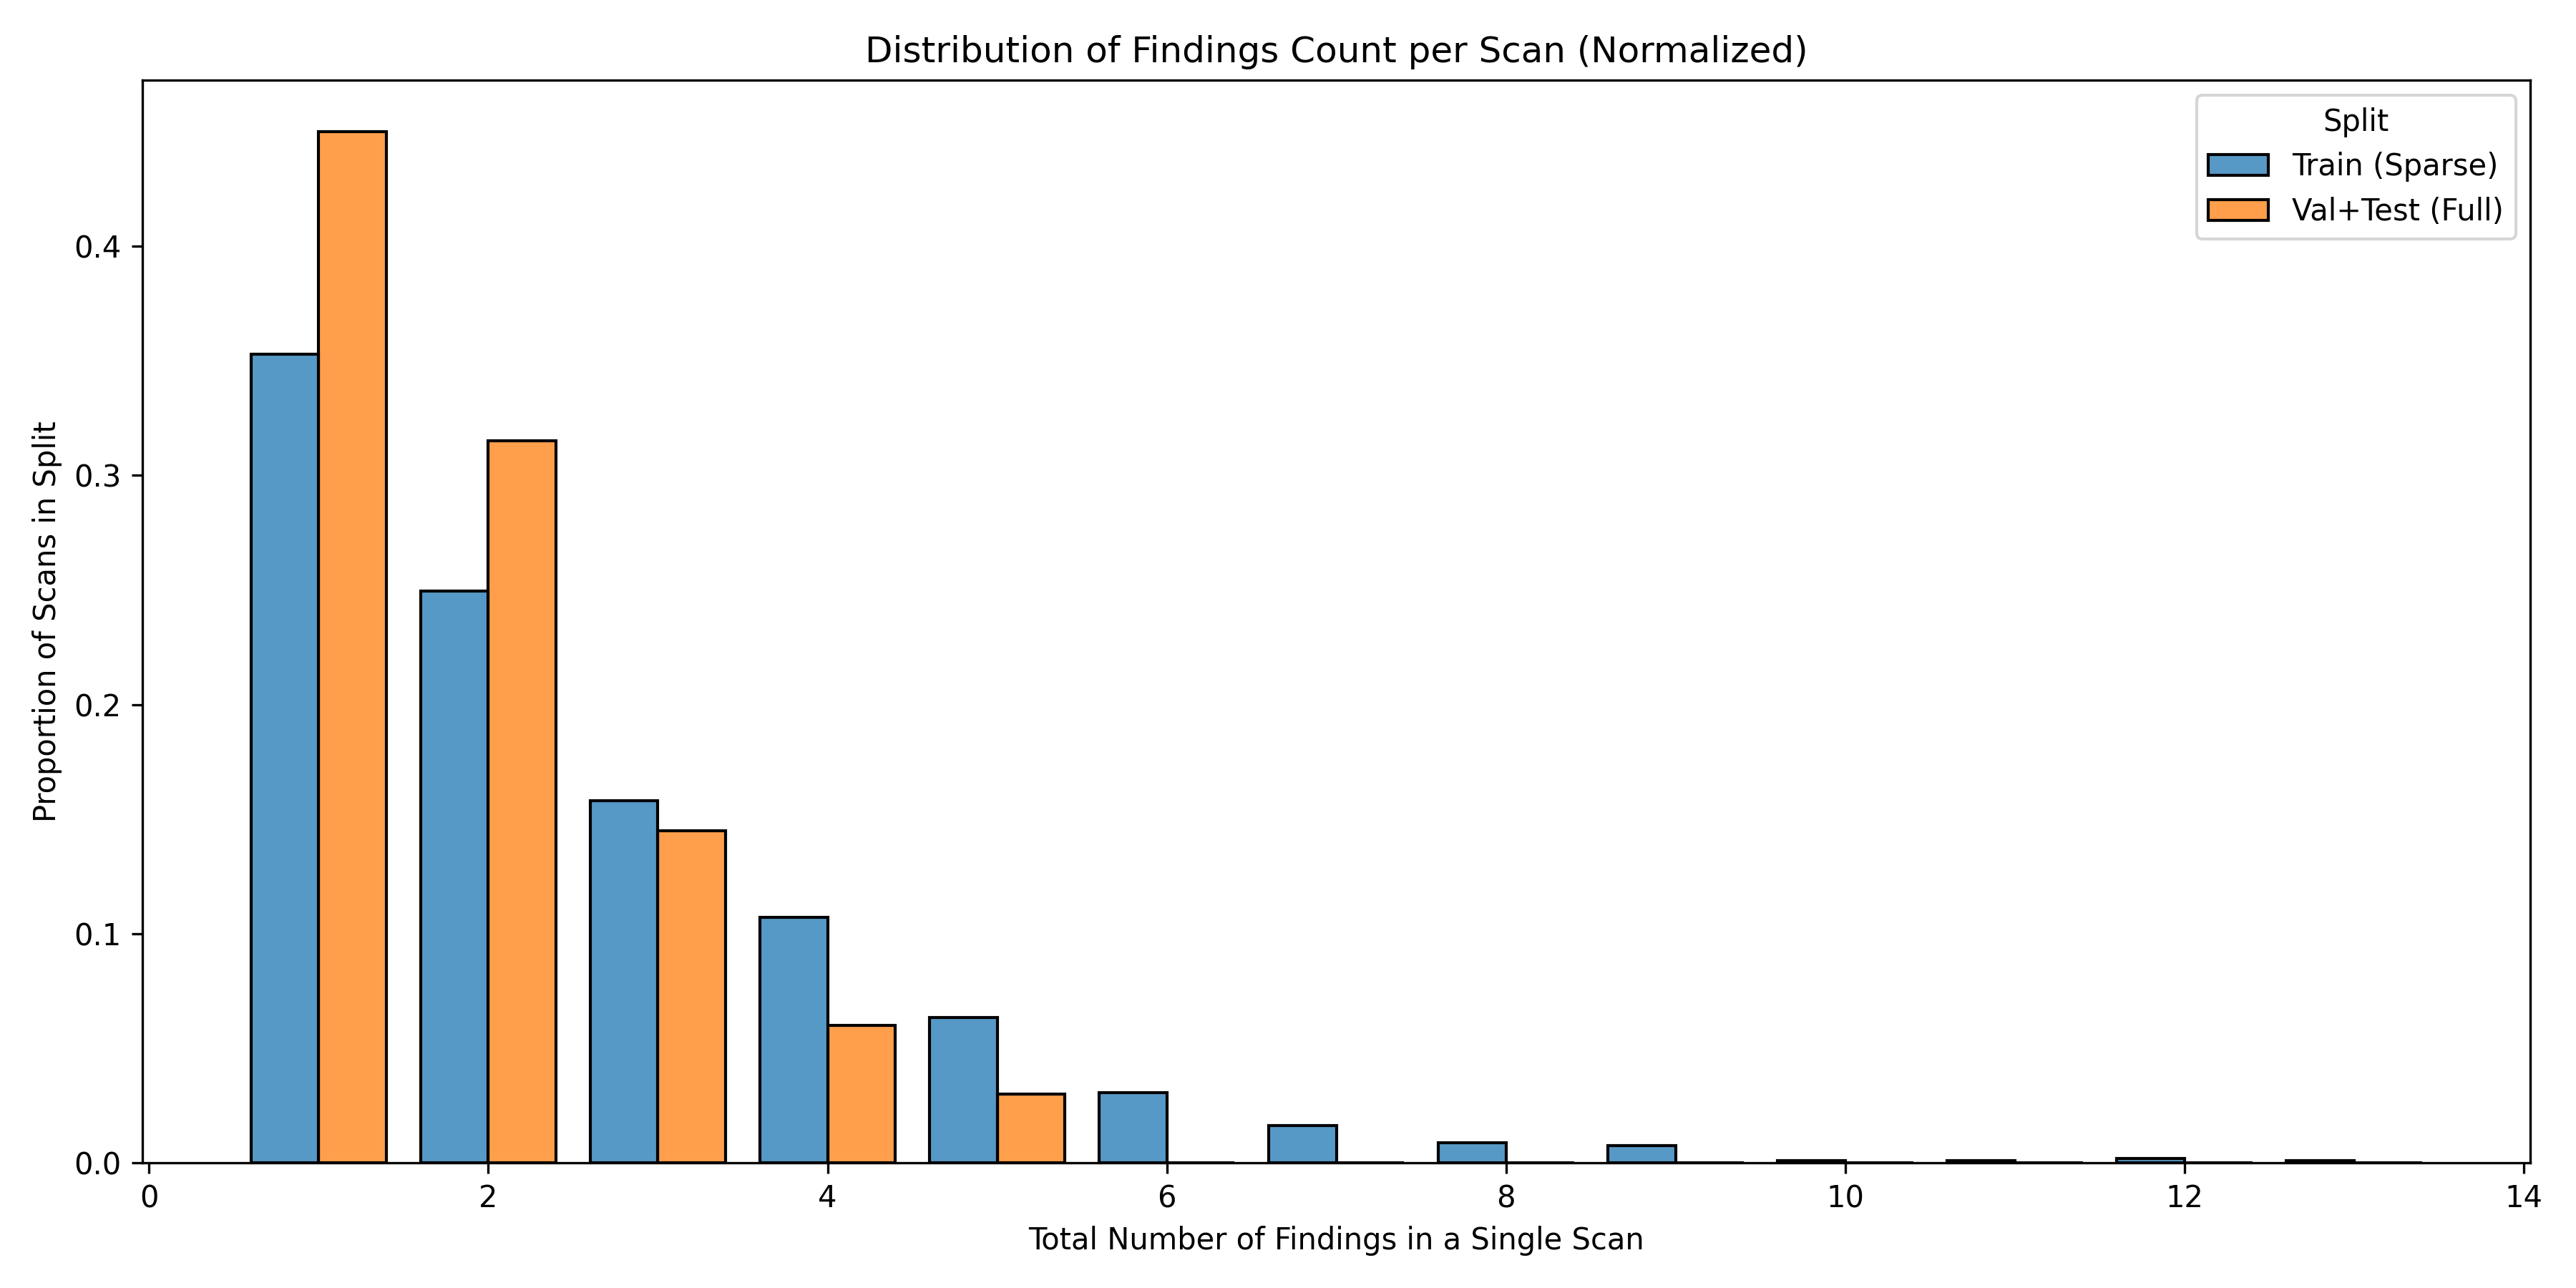
\includegraphics[width=\textwidth]{fig/exp001_findings_per_scan.png}
    \caption{Distribution of findings per CT scan record.}
\end{subfigure}
\caption{Experiment 001 dataset composition and category frequency profiling.}
\label{fig:exp001_composition}
\end{figure}

\subsection{Scan-Level Pathology Co-Occurrence Structure}
To understand multi-finding pathology dependence across multi-label CT volumes, we computed the $14 \times 14$ scan-level conditional probability co-occurrence matrix $P(c_j \text{ present} \mid c_i \text{ present})$, visualized in Figure~\ref{fig:cooccurrence_heatmap}.

\begin{figure}[H]
\centering

\includegraphics[width=0.82\textwidth]{fig/exp001_cooccurrence_heatmap.png}
\caption{Scan-level $14 \times 14$ pathology co-occurrence probability matrix $P(c_j \text{ present} \mid c_i \text{ present})$ across multi-label CT scans.}
\label{fig:cooccurrence_heatmap}
\end{figure}

High co-occurrence is observed between dependent pathologies, such as Pleural effusion (\texttt{2e}) co-occurring with Atelectasis/consolidation (\texttt{2b}) at $P(\text{Atelectasis} \mid \text{Effusion}) = 0.600$, and Honeycombing (\texttt{2f}) co-occurring with Atelectasis/consolidation (\texttt{2b}) and Pulmonary nodules/masses (\texttt{2d}) at $P = 0.467$ ($7/15$ co-occurring scans).

\subsection{Patient Hierarchy \& Cross-Split Leakage Audit}
Parsing patient ID conventions across all 3,078 physical NIfTI scan acquisitions (2,578 Train / 200 Val / 300 Test) reveals a 3-tier structure comprising 3,063 unique physical patients. The arithmetic checks out exactly:
\begin{equation}
N_{\text{unique}} = 2,603 \text{ (Train)} + 190 \text{ (Val)} + 281 \text{ (Test)} - 11 \text{ (Overlaps)} = 3,063 \text{ unique patients}.
\end{equation}

Our systematic cross-split patient leakage audit identified:
\begin{itemize}
    \item \textbf{Train-Val Patient Overlap}: 2 overlapping patients (\texttt{['1841', '2936']}). Flagged for validation isolation to prevent optimistic validation bias.
    \item \textbf{Train-Test Patient Overlap}: 4 overlapping patients (\texttt{['302', '3357', '3675', '39']}). Noted for evaluation integrity auditing.
    \item \textbf{Val-Test Patient Overlap}: 5 overlapping patients (\texttt{['13119', '13278', '13479', '13492', '13583']}). Recorded in validation hierarchy metadata.
\end{itemize}

Val-Test patient overlap presents the highest risk to evaluation integrity: if model tuning hyper-parameters implicitly exploit patient-level anatomical features learned during validation on these 5 patients, performance on the corresponding Test scans may be artificially inflated. Strict split isolation is mandatory during local validation.

\bigskip

\section{Exp 002: Free-Text Prompt Syntax \& NLP Text Shift Analysis}

\subsection{Validation Prompt Text Shift (Cases 1--50 vs.\ Cases 51--200)}
Experiment 002 evaluates the clinical text characteristics across all 8,650 prompts in the benchmark. Critically, we identified a significant syntactic prompt shift between the first 50 validation cases (used in the original VoxTell paper benchmark~\cite{luo2025voxtell}) and cases 51--200 (the expanded MICCAI competition validation set), detailed in Table~\ref{tab:nlp_shift}.

\begin{table}[H]
\centering
\caption{NLP syntactic prompt shift analysis on Validation Cases 1--50 vs.\ Cases 51--200.}
\label{tab:nlp_shift}
\begin{adjustbox}{max width=\linewidth}
\small
\setlength{\tabcolsep}{5pt}
\begin{tabular}{lccccc}
\toprule
\textbf{Metric / Parameter} & \makecell{\textbf{Cases 1--50}\\\textbf{(Paper)}} & \makecell{\textbf{Cases 51--200}\\\textbf{(MICCAI)}} & \textbf{Ratio} & \makecell{\textbf{Percentage}\\\textbf{Change}} & \textbf{Combined Val} \\
\midrule
Total Finding Prompts & 115 & 266 & 2.31x & +131.3\% & 381 \\
Total Word Tokens & 1,263 & 3,193 & 2.53x & +152.8\% & 4,456 \\
Mean Word Count per Prompt & 10.98 words & 12.00 words & 1.09x & +9.3\% & 11.70 words \\
Max Word Count in Prompt & 21 words & \textbf{35 words} & \textbf{1.67x} & \textbf{+66.7\%} & 35 words \\
Mean Character Length & 70.0 chars & 80.0 chars & 1.14x & +14.3\% & 76.98 chars \\
Prompts with Comma Punctuation & 11.30\% & \textbf{23.68\%} & \textbf{2.10x} & \textbf{+12.38\% pt} & 19.95\% \\
Type-Token Ratio (TTR, Naive)$^*$ & 0.1544 & 0.0817 & 0.53x & -47.1\% & 0.0741 \\
LN-TTR (1,000 Tokens Monte Carlo) & 0.1740 & 0.1651 & 0.95x & -5.11\% & 0.1746 \\
\bottomrule
\end{tabular}
\end{adjustbox}
\vspace{2mm}
\raggedright \footnotesize $^*$Naive TTR is inherently biased by corpus token size due to Heaps' Law (as total token count expands, vocabulary saturation reduces naive TTR). Log-Normal TTR (LN-TTR) controls for corpus length, confirming stable lexicon diversity.
\end{table}

Prompts in cases 51--200 exhibit longer, highly clause-heavy sentences with a 1.67x spike in maximum word length (up to 35 words) and more than double the comma punctuation frequency (23.68\% vs.\ 11.30\%).

\subsection{Subword Tokenization Dynamics, Spatial Directives \& Hedging}
\begin{itemize}
    \item \textbf{Subword BPE Tokenization Dynamics}: Tokenizing prompts with standard medical BERT/CLIP tokenizers yields an average of $13.75$ subword BPE tokens per prompt compared to $10.21$ raw words, representing a $+34.7\%$ BPE tokenization expansion factor ($1.347\text{x}$). Maximum prompt token length remains strictly below 128 tokens across all splits, resulting in a $0.0\%$ context truncation rate.
    \item \textbf{Spatial Locators}: 64.39\% of all prompts contain explicit anatomical position locators (\textit{"right"}, \textit{"upper lobe"}, \textit{"subpleural"}, \textit{"peribronchovascular"}).
    \item \textbf{Diagnostic Hedging}: Hedging language (\textit{"possible"}, \textit{"equivocal"}, \textit{"cannot be excluded"}) was identified in only 0.38\% of prompts (33 prompts dataset-wide), demonstrating that hedging noise is negligible and does not require complex NLP text pruning.
\end{itemize}

\bigskip

\section{Exp 003: Anatomical Spatial Density Priors \& 4-Tier Taxonomy}

\subsection{Canonical RAS Coordinate Centroids \& 4-Tier Taxonomy}
Experiment 003 resamples all 3D ground-truth masks into a canonical $128 \times 128 \times 128$ RAS spatial coordinate grid to compute canonical 3D spatial probability density volumes $\mathbf{P}_{\text{train}}, \mathbf{P}_{\text{val}} \in \mathbb{R}^{128 \times 128 \times 128}$ and average spatial centroids $\mathbf{c} = (RL, AP, IS) \in [0.0, 1.0]^3$. 

To quantify 3D spatial probability density alignment across splits, Cosine Similarity $S_{\text{cos}}$ is calculated as the normalized Frobenius inner product between the resampled 3D spatial probability density maps:
\begin{equation}
S_{\text{cos}} = \frac{\langle \mathbf{P}_{\text{train}}, \mathbf{P}_{\text{val}} \rangle_F}{\|\mathbf{P}_{\text{train}}\|_F \|\mathbf{P}_{\text{val}}\|_F} = \frac{\sum_{\mathbf{x}} P_{\text{train}}(\mathbf{x}) P_{\text{val}}(\mathbf{x})}{\sqrt{\sum_{\mathbf{x}} P_{\text{train}}(\mathbf{x})^2} \sqrt{\sum_{\mathbf{x}} P_{\text{val}}(\mathbf{x})^2}},
\end{equation}
while Centroid Distance Shift $\Delta d$ measures the Euclidean distance between mean centroids: $\Delta d = \|\mathbf{c}_{\text{val}} - \mathbf{c}_{\text{train}}\|_2$.

Based on population 3D spatial probability density distributions $\mathbf{P}_{\text{train}}(\mathbf{x})$ (visualized in Figure~\ref{fig:exp003_priors}) and anatomical clinical domain priors, findings are categorized into a 4-tier spatial prior taxonomy detailed in Table~\ref{tab:spatial_centroids}:
\begin{enumerate}
    \item \textbf{Apical Dominant Prior} (\texttt{1c} Emphysema): Population 3D probability density is heavily concentrated in superior lung zones ($IS = 0.667$ in Train, $IS = 0.789$ in Val).
    \item \textbf{Basal / Dependent Prior} (\texttt{2b} Atelectasis, \texttt{2e} Pleural effusion, \texttt{2f} Honeycombing$^*$): Density maps localize in inferior and posterior gravitational regions ($IS \approx 0.416$--$0.491, AP \approx 0.314$).
    \item \textbf{Hilar / Peribronchial Prior} (\texttt{1a} Bronchial wall thickening, \texttt{1b} Bronchiectasis): Density maps cluster tightly around central bronchovascular tree structures ($RL \approx 0.508$--$0.510, IS \approx 0.541$--$0.545$).
    \item \textbf{Isotropic / Parenchymal Prior} (\texttt{2d} Nodules, \texttt{1e} Micronodules, \texttt{2c} GGO, \texttt{2a} Linear opacities): Broad parenchymal distribution across pulmonary fields without focal gravitational or apical confinement ($IS \approx 0.52$--$0.56, RL \approx 0.47$--$0.54$).
\end{enumerate}

\begin{table}[H]
\centering
\caption{Canonical 3D RAS spatial centroids $(RL, AP, IS) \in [0.0, 1.0]^3$, centroid distance shift $\Delta d$, 3D spatial density cosine similarity $S_{cos}$, and 4-tier spatial density prior taxonomy across all 14 finding categories.}
\label{tab:spatial_centroids}
\begin{adjustbox}{max width=\linewidth}
\small
\setlength{\tabcolsep}{3.5pt}
\begin{tabular}{lcccccc}
\toprule
\textbf{Code} & \textbf{Finding Category} & \makecell{\textbf{Train Centroid}\\\textbf{$(RL, AP, IS)$}} & \makecell{\textbf{Val Centroid}\\\textbf{$(RL, AP, IS)$}} & $\Delta d$ & $S_{cos}$ & \makecell{\textbf{Spatial Prior}\\\textbf{Taxonomy}} \\
\midrule
\texttt{1a} & Bronchial wall thickening & $(0.508, 0.439, 0.541)$ & $(0.495, 0.491, 0.478)$ & 0.0825 & 0.0412 & Hilar / Peribronchial \\
\texttt{1b} & Bronchiectasis & $(0.510, 0.449, 0.545)$ & $(0.471, 0.489, 0.548)$ & 0.0563 & 0.2059 & Hilar / Peribronchial \\
\texttt{1c} & Emphysema & $(0.504, 0.442, 0.667)$ & $(0.466, 0.533, 0.789)$ & 0.1566 & 0.1756 & \textbf{Apical Dominant} \\
\texttt{1d} & Septal thickening & $(0.519, 0.420, 0.563)$ & $(0.519, 0.474, 0.469)$ & 0.1092 & 0.2228 & Isotropic / Parenchymal \\
\texttt{1e} & Micronodules & $(0.517, 0.422, 0.537)$ & $(0.468, 0.499, 0.580)$ & 0.1007 & 0.1111 & Isotropic / Parenchymal \\
\texttt{1f} & Other non-focal & $(0.501, 0.426, 0.545)$ & $(0.404, 0.488, 0.479)$ & 0.1327 & 0.0671 & Isotropic / Parenchymal \\
\texttt{2a} & Linear opacities & $(0.474, 0.500, 0.535)$ & $(0.563, 0.492, 0.537)$ & 0.0886 & 0.2562 & Isotropic / Parenchymal \\
\texttt{2b} & Atelectasis / consolidation & $(0.503, 0.433, 0.491)$ & $(0.531, 0.507, 0.416)$ & 0.1084 & 0.3275 & \textbf{Basal / Dependent} \\
\texttt{2c} & Ground-glass opacity & $(0.510, 0.407, 0.519)$ & $(0.497, 0.560, 0.442)$ & 0.1711 & 0.4432 & Isotropic / Parenchymal \\
\texttt{2d} & Pulmonary nodules / masses & $(0.540, 0.452, 0.556)$ & $(0.466, 0.521, 0.554)$ & 0.1012 & 0.0268 & Isotropic / Parenchymal \\
\texttt{2e} & Pleural effusion / thickening & $(0.535, 0.314, 0.484)$ & $(0.461, 0.539, 0.431)$ & 0.2426 & 0.5032 & \textbf{Basal / Dependent} \\
\texttt{2f} & Honeycombing$^*$ & $(0.457, 0.482, 0.498)$ & -- & -- & -- & \textbf{Basal / Dependent} \\
\texttt{2g} & Pneumothorax & $(0.497, 0.516, 0.522)$ & $(0.304, 0.443, 0.622)$ & 0.2293 & 0.0717 & Isotropic / Parenchymal \\
\texttt{2h} & Other focal & $(0.521, 0.442, 0.536)$ & $(0.513, 0.488, 0.578)$ & 0.0633 & 0.0101 & Isotropic / Parenchymal \\
\bottomrule
\end{tabular}
\end{adjustbox}
\vspace{2mm}
\raggedright \footnotesize $^*$Honeycombing (\texttt{2f}) contains 0 instances in the Validation split ($N_{\text{val}}=0$); its spatial prior taxonomy is assigned based on Train split spatial distribution ($N_{\text{train}}=16$) and clinical domain priors.
\end{table}

\begin{figure}[H]
\centering
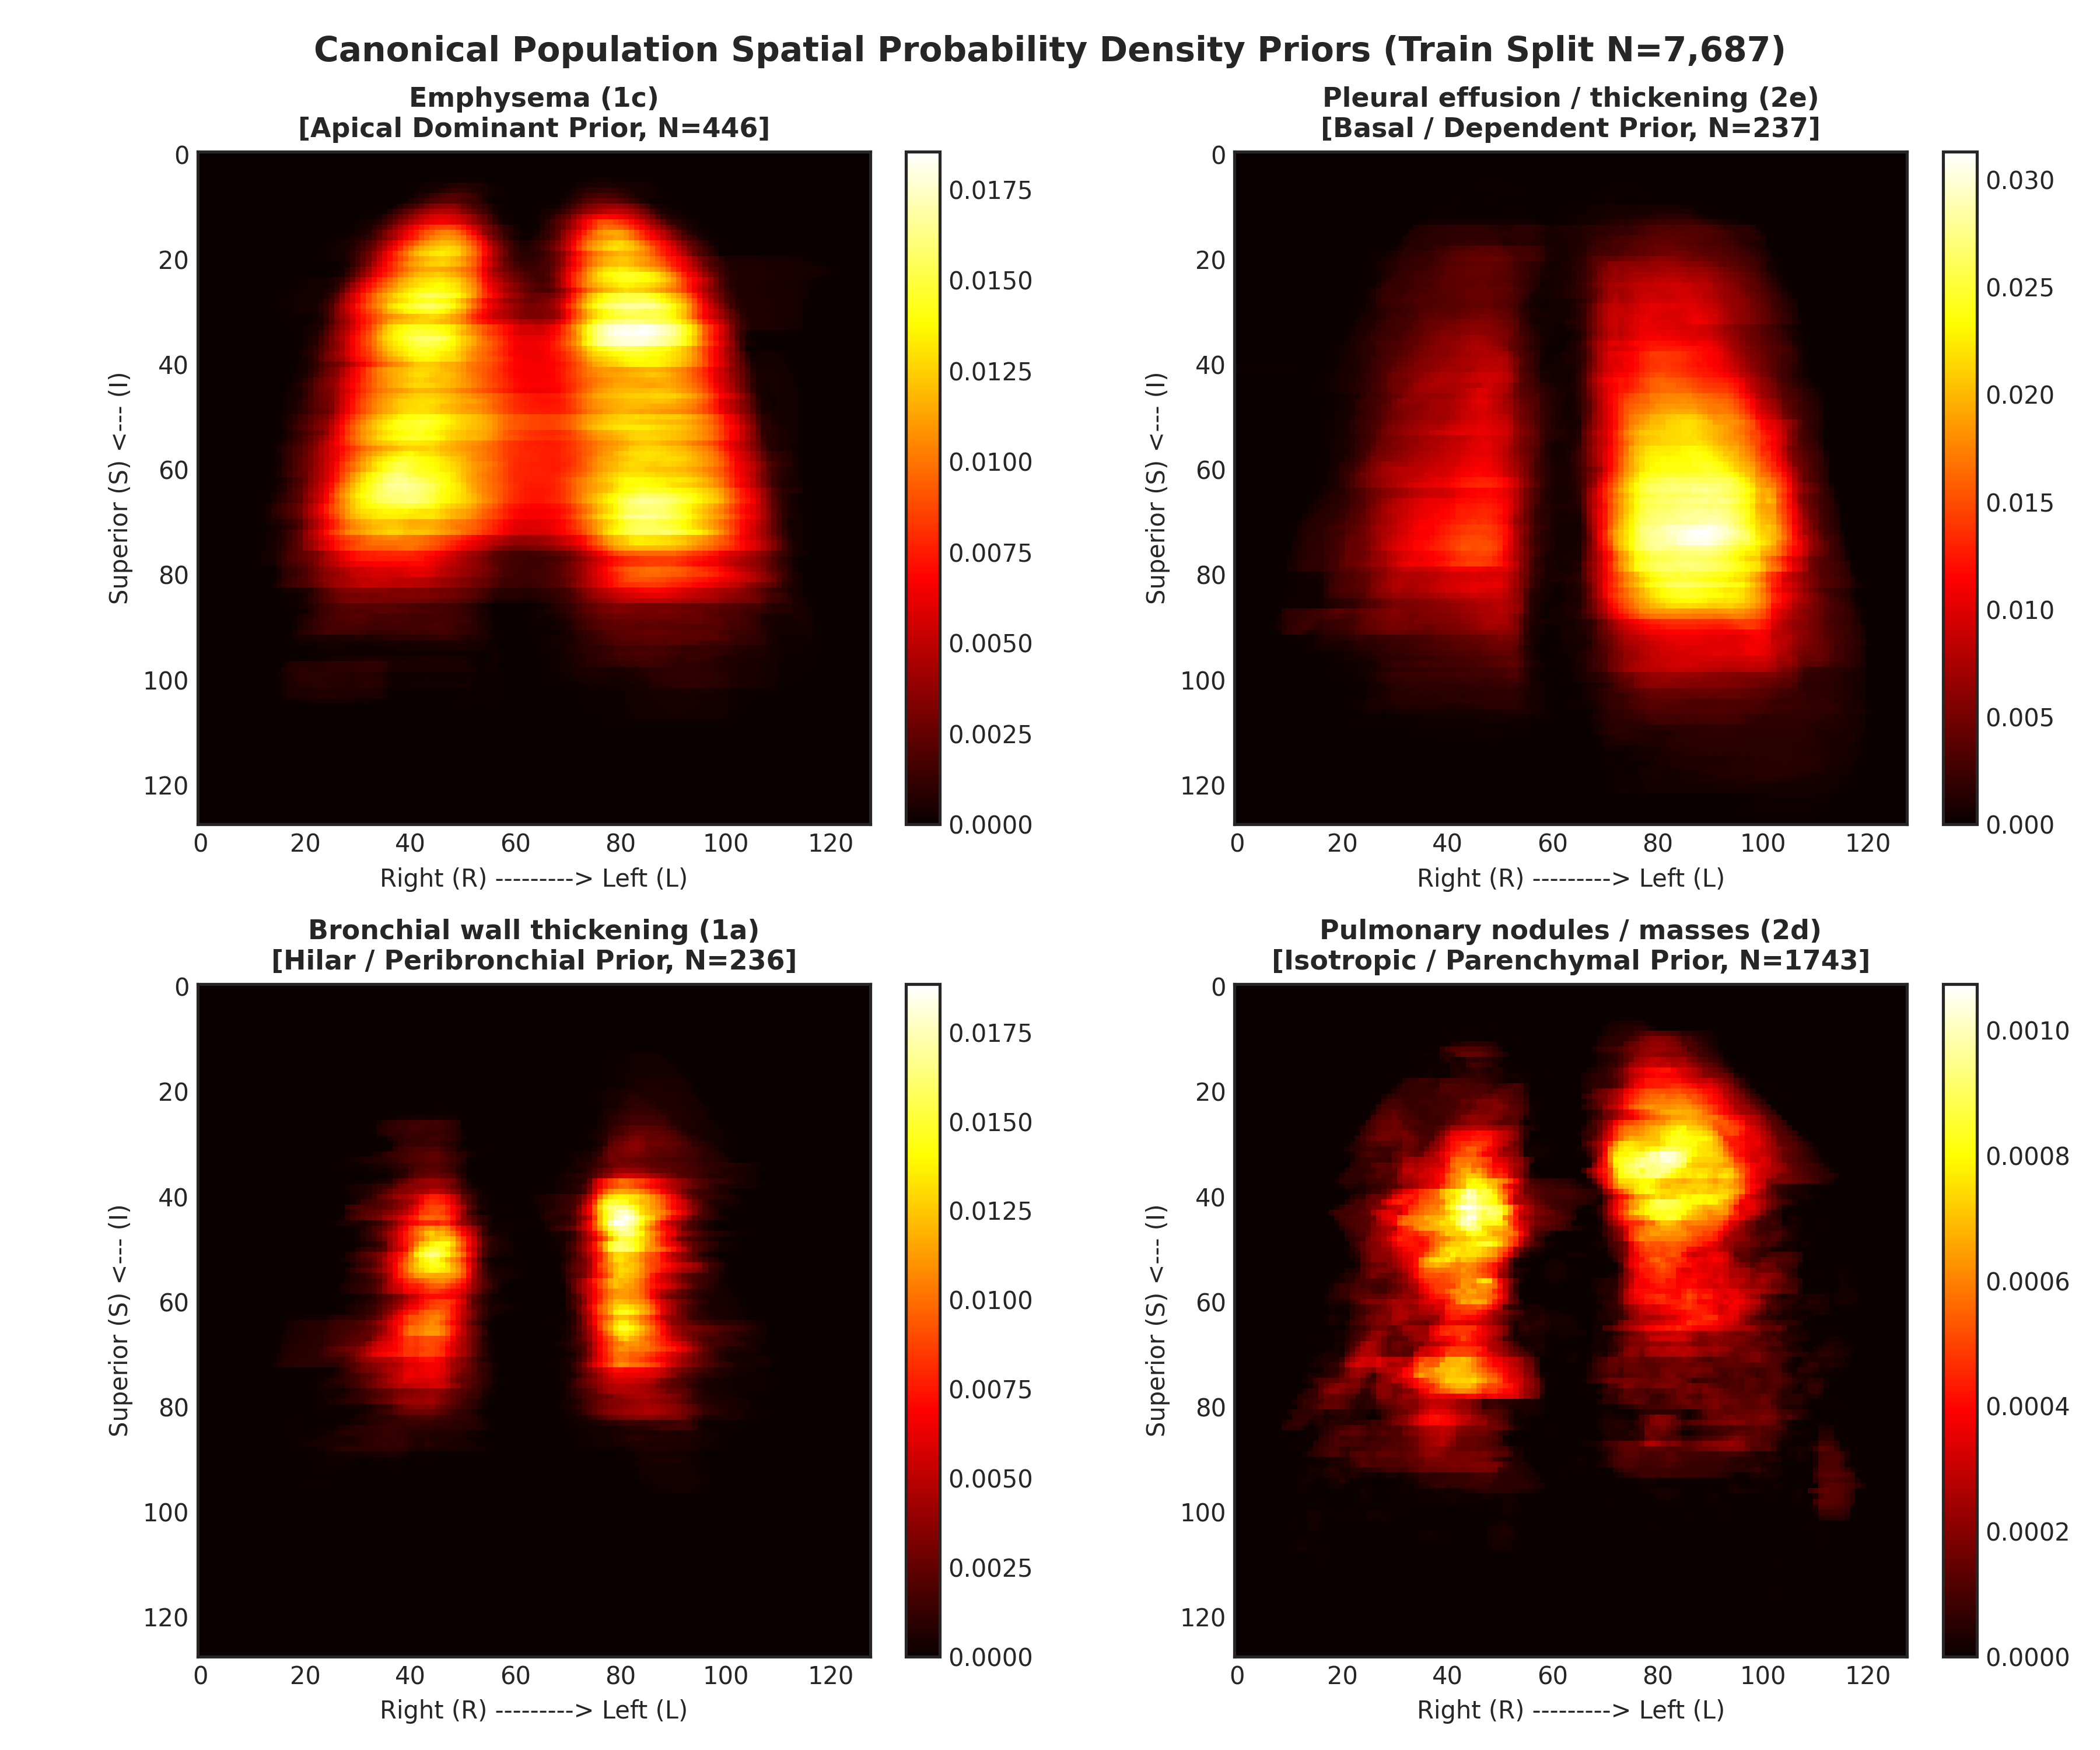
\includegraphics[width=0.95\textwidth]{fig/exp003_population_spatial_priors_4panel.png}
\caption{Canonical 3D spatial probability density priors across key taxonomy categories (Coronal projections, $128 \times 128 \times 128$ RAS grid).}
\label{fig:exp003_priors}
\end{figure}

High spatial density stability is observed in focal pathologies (e.g., nodules $\Delta d = 0.101$). Conversely, dependent and pleural pathologies (Pleural effusion $\Delta d = 0.243$, Pneumothorax $\Delta d = 0.229$) exhibit noticeable centroid shifts between splits due to anatomical gravity variation and sparse vs.\ exhaustive sampling, highlighting the need for spatial prior masking during search space pruning.

\bigskip

\section{Exp 004: Hounsfield Unit (HU) Radiodensity Attenuation Profiling}

Experiment 004 extracts physical Hounsfield Unit (HU) intensity values inside ground-truth pathology masks vs.\ surrounding healthy parenchyma across 3,192 CT volumes.

\begin{figure}[H]
\centering
\begin{subfigure}[b]{0.48\textwidth}
    \centering
    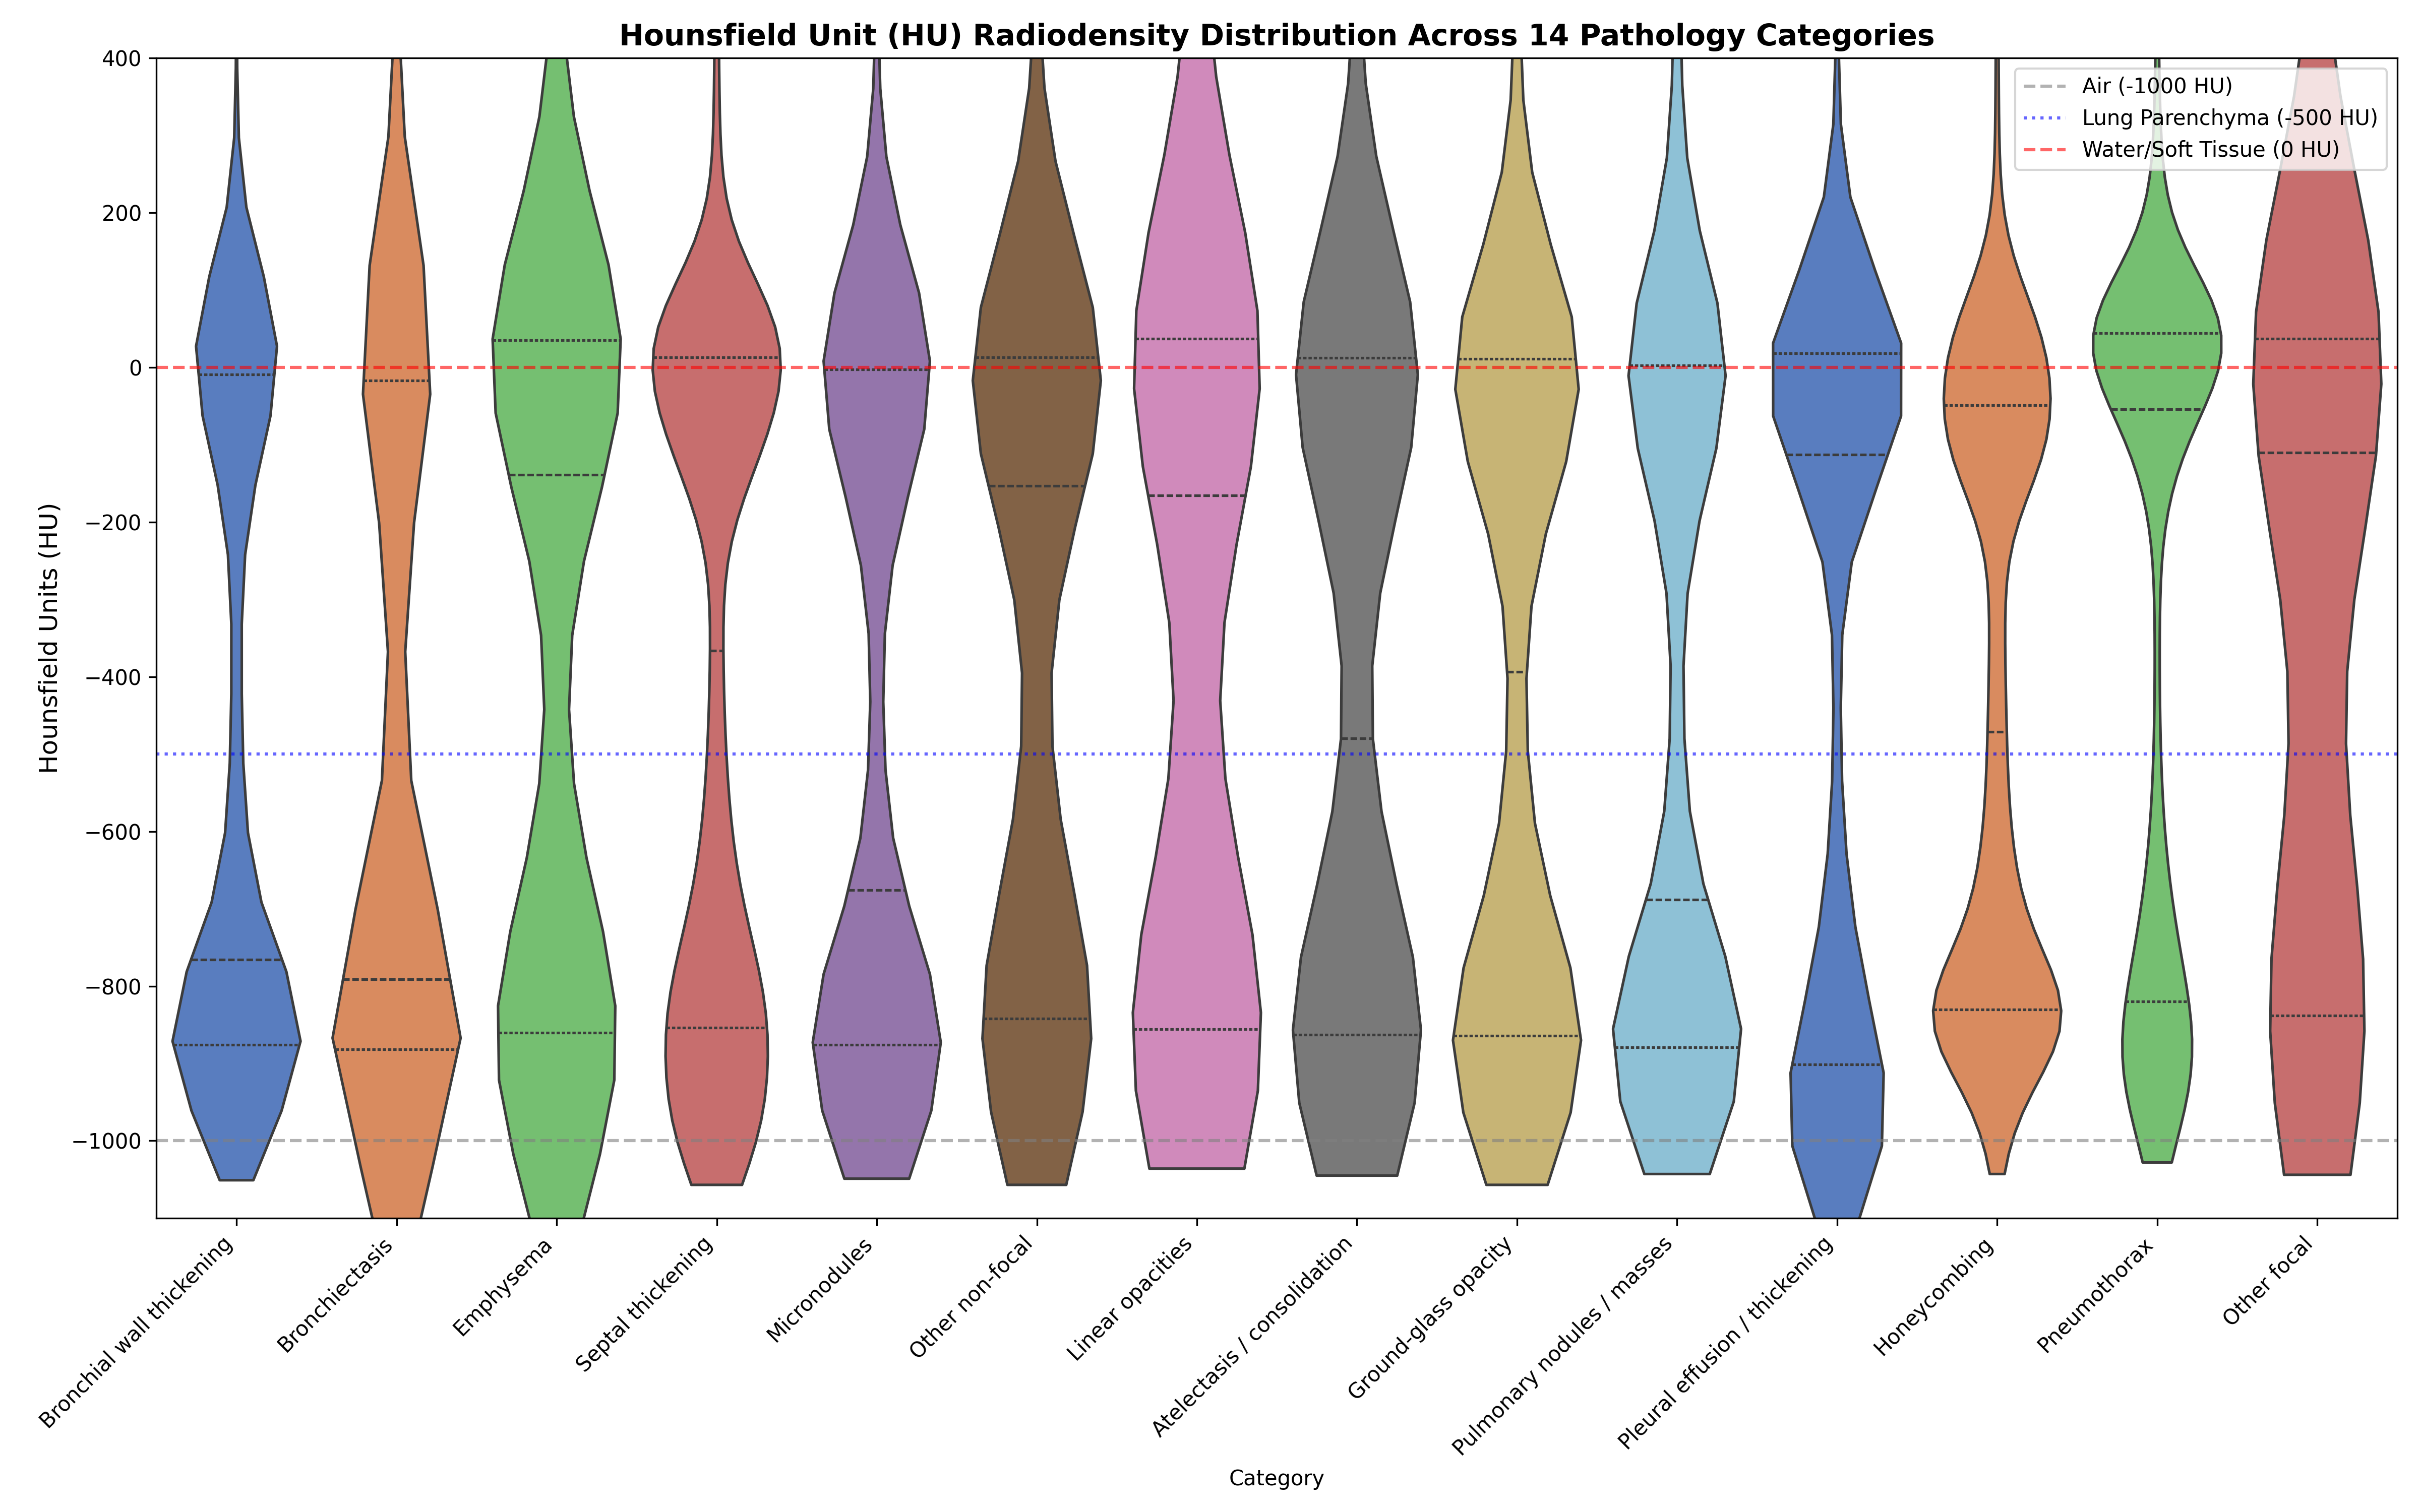
\includegraphics[width=\textwidth]{fig/exp004_hu_distribution_violin.png}
    \caption{HU radiodensity violin distributions per category.}
\end{subfigure}
\hfill
\begin{subfigure}[b]{0.48\textwidth}
    \centering
    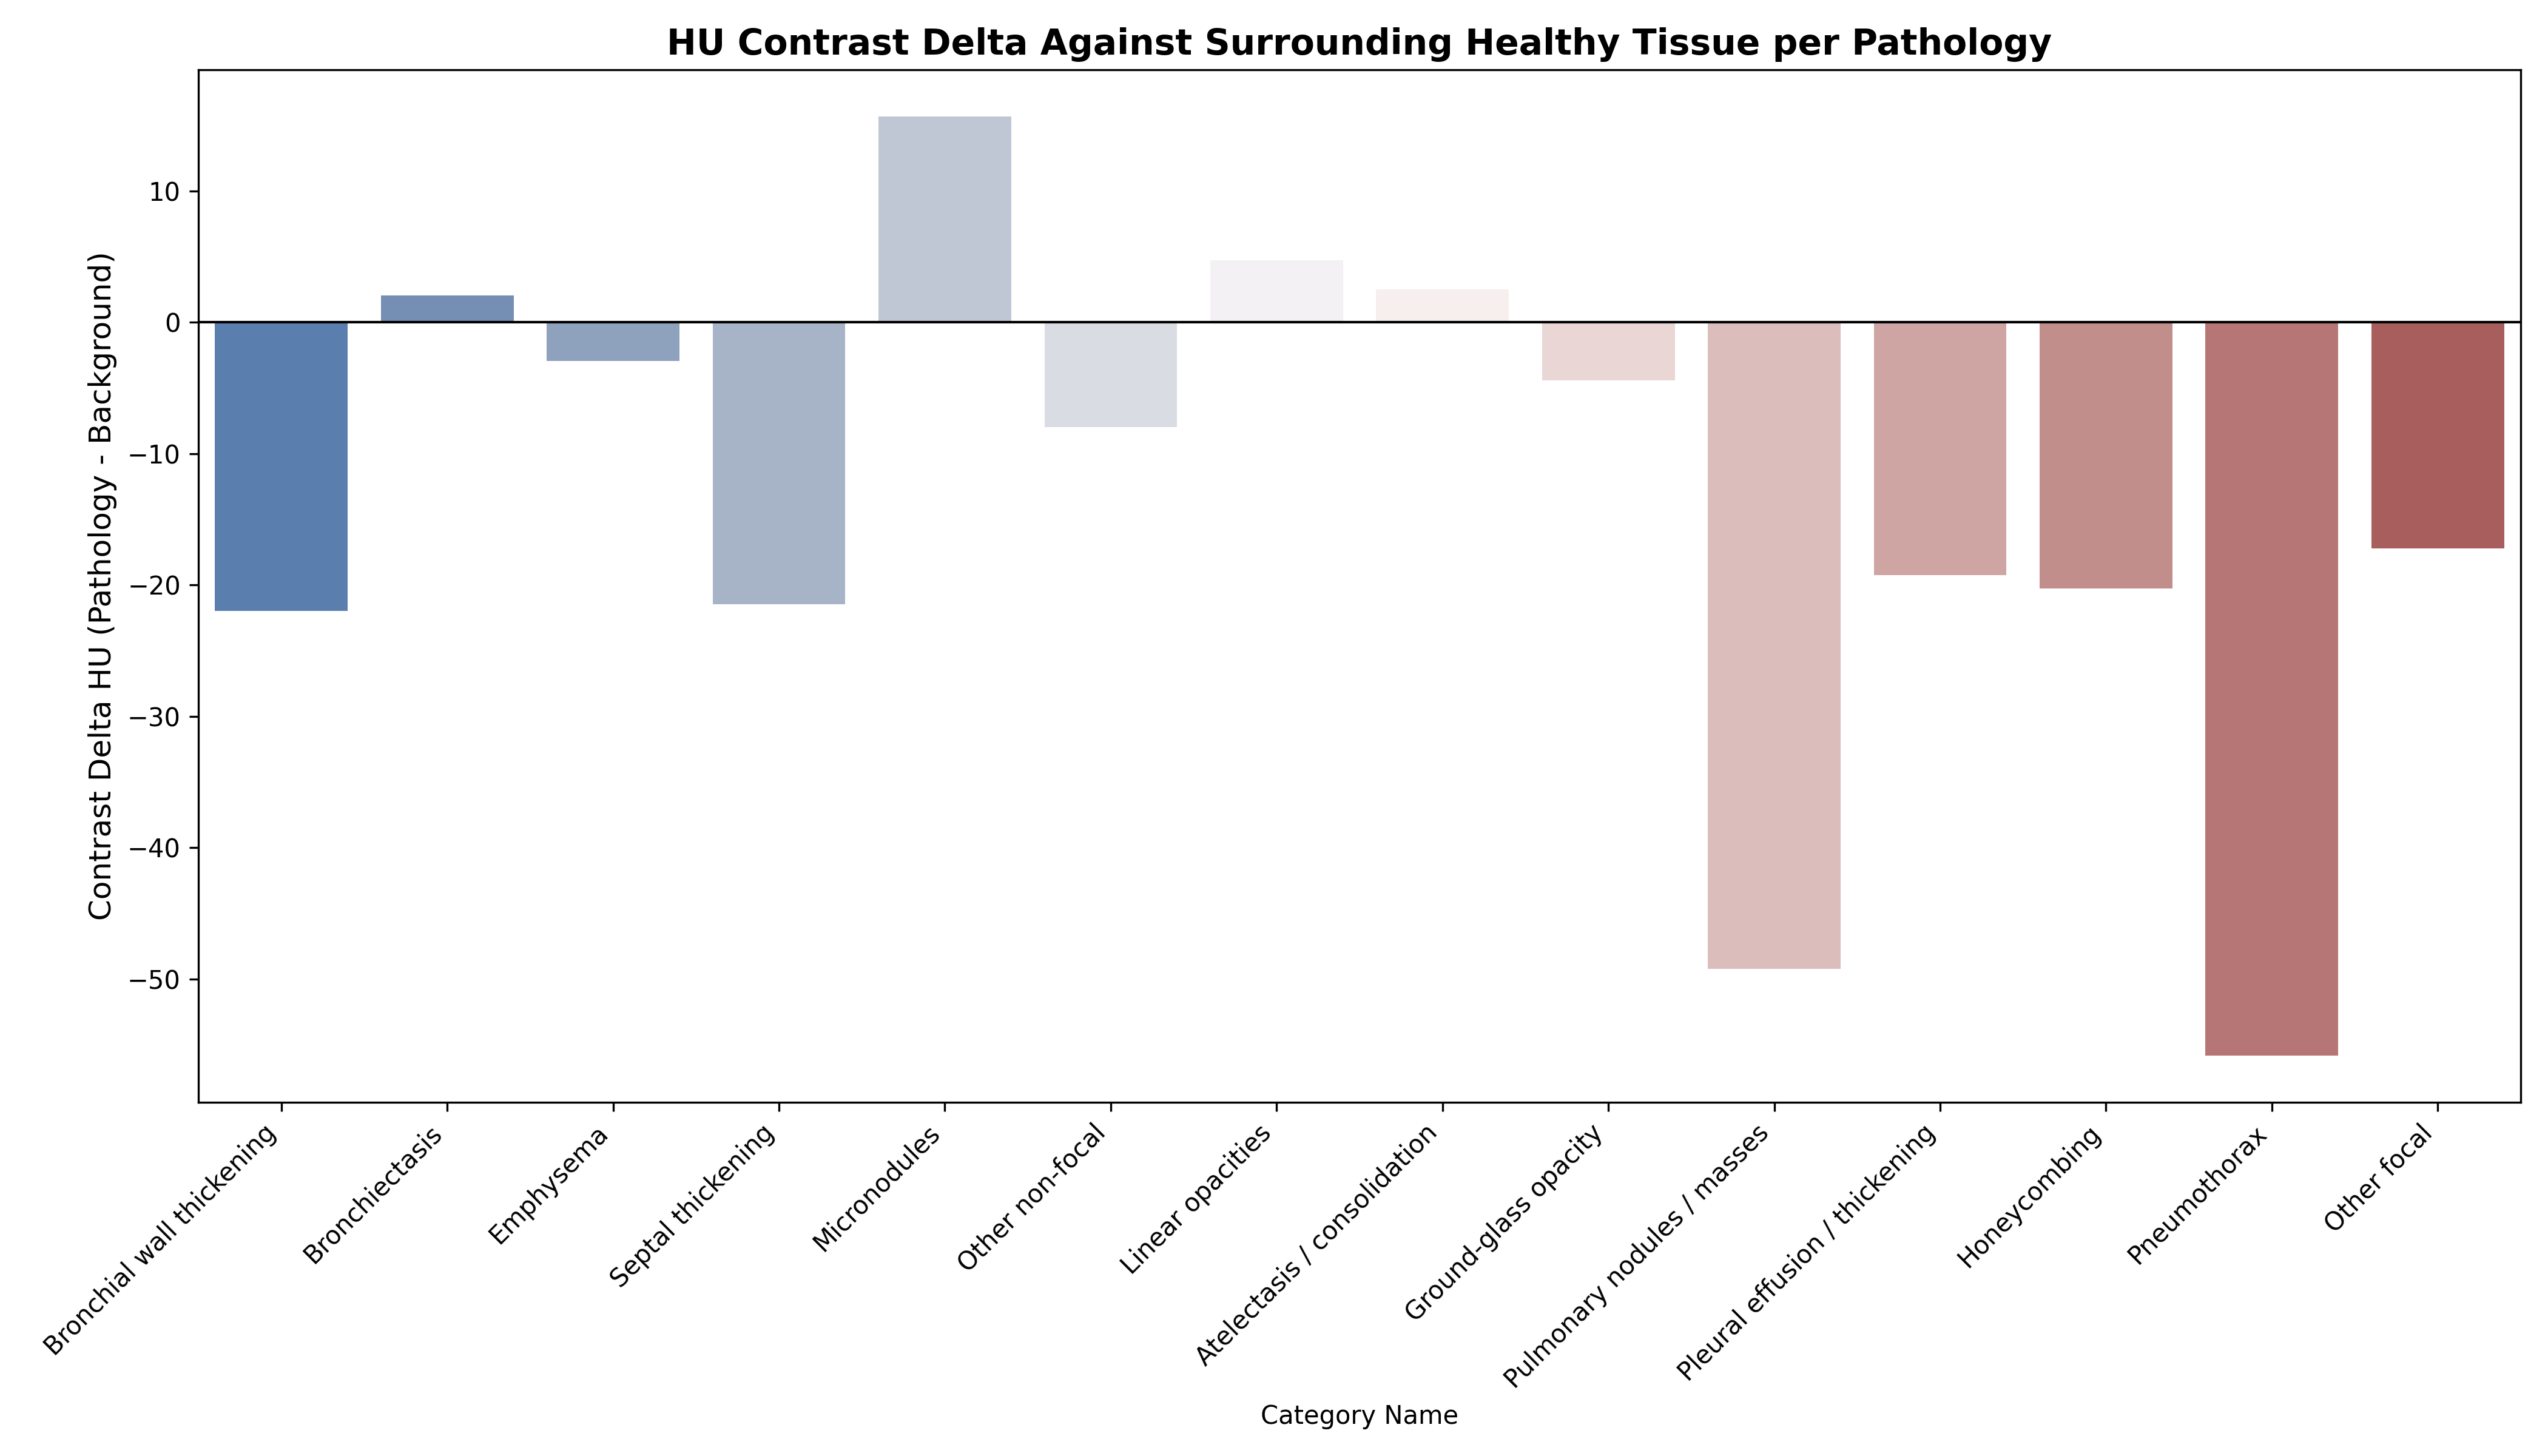
\includegraphics[width=\textwidth]{fig/exp004_hu_contrast_delta_barplot.png}
    \caption{Contrast delta $\Delta \text{HU}$ (Pathology vs.\ Background).}
\end{subfigure}
\caption{Hounsfield Unit (HU) radiodensity attenuation profiling across all 14 categories.}
\label{fig:exp004_hu}
\end{figure}

\begin{table}[H]
\centering
\caption{Category-level Hounsfield Unit (HU) attenuation statistics, mask sample counts ($N_{\text{masks}}$), contrast deltas ($\Delta \text{HU} = \text{Mean HU} - \text{Bg Mean HU}$), and recommended windowing bounds \texttt{[min\_HU, max\_HU]}.}
\label{tab:hu_stats}
\begin{adjustbox}{max width=\linewidth}
\small
\setlength{\tabcolsep}{4pt}
\begin{tabular}{lm{3.2cm}cccccc}
\toprule
\textbf{Cat Code} & \textbf{Category Name} & \textbf{$N_{\text{masks}}$} & \textbf{Mean HU} & \textbf{P5 HU} & \textbf{P95 HU} & \makecell{\textbf{Contrast}\\\textbf{$\Delta\text{HU}$}} & \makecell{\textbf{Rec Window}\\\textbf{[Min, Max]}} \\
\midrule
\texttt{1a} & Bronchial wall thickening & 239 & -486.35 & -933.0 & +69.0 & -21.98 & [-933.0, +69.0] \\
\texttt{1b} & Bronchiectasis & 293 & -477.93 & -934.0 & +86.0 & +1.93 & [-934.0, +86.0] \\
\texttt{1c} & Emphysema & 463 & -307.95 & -992.0 & +251.0 & -3.11 & [-992.0, +251.0] \\
\texttt{1d} & Septal thickening & 200 & -406.38 & -1001.0 & +121.0 & -21.23 & [-1001.0, +121.0] \\
\texttt{1e} & Micronodules & 325 & -427.36 & -998.0 & +101.0 & +15.16 & [-998.0, +101.0] \\
\texttt{1f} & Other non-focal & 154 & -334.71 & -987.0 & +98.0 & -8.61 & [-987.0, +98.0] \\
\texttt{2a} & Linear opacities & 1,189 & -286.55 & -992.0 & +399.0 & +4.68 & [-992.0, +399.0] \\
\texttt{2b} & Atelectasis / consolidation & 1,416 & -341.35 & -995.0 & +129.0 & +2.43 & [-995.0, +129.0] \\
\texttt{2c} & Ground-glass opacity & 1,567 & -375.11 & -995.0 & +137.0 & -4.51 & [-995.0, +137.0] \\
\texttt{2d} & Pulmonary nodules / masses & 1,875 & -427.06 & -995.0 & +194.0 & -49.15 & [-995.0, +194.0] \\
\texttt{2e} & Pleural effusion / thickening & 248 & -368.59 & -1007.0 & +135.0 & -19.37 & [-1007.0, +135.0] \\
\texttt{2f} & Honeycombing & 16 & -420.45 & -905.0 & +83.0 & -18.07 & [-905.0, +83.0] \\
\texttt{2g} & Pneumothorax & 19 & -306.85 & -961.0 & +148.0 & -54.68 & [-961.0, +148.0] \\
\texttt{2h} & Other focal & 64 & -156.62 & -915.0 & +201.0 & -16.21 & [-915.0, +201.0] \\
\bottomrule
\end{tabular}
\end{adjustbox}
\end{table}

Key radiodensity observations:
\begin{itemize}
    \item \textbf{Radiodensity Attenuation Range}: Mean attenuation ranges from \texttt{2h} Other focal ($-156.62\text{ HU}$) and \texttt{2a} Linear opacities ($-286.55\text{ HU}$) to air-filled airway wall pathologies like \texttt{1a} Bronchial wall thickening ($-486.35\text{ HU}$) and \texttt{1b} Bronchiectasis ($-477.93\text{ HU}$). Low sample size categories (\texttt{2f} Honeycombing $N=16$, \texttt{2g} Pneumothorax $N=19$) exhibit higher statistical variance.
    \item \textbf{Contrast Deltas ($\Delta \text{HU}$)}: Soft-tissue focal lesions (micronodules $+15.16\text{ HU}$, linear opacities $+4.68\text{ HU}$, consolidation $+2.43\text{ HU}$) exhibit positive contrast deltas against immediate background, whereas nodules ($-49.15\text{ HU}$) and pneumothorax ($-54.68\text{ HU}$) show distinct negative boundary deltas against surrounding parenchyma.
    \item \textbf{Optimal Windowing Bounds}: Preprocessing CT volumes with category-tailored intensity windowing \texttt{[min\_HU, max\_HU]} (e.g. \texttt{[-995, +194] HU} for nodules vs \texttt{[-933, +69] HU} for bronchial thickening) enhances feature contrast during model training.
\end{itemize}

\bigskip

\section{Exp 005: 3D Morphological Topology \& Size Thresholds}

Experiment 005 profiles 3D connected component morphology, geometric sphericity index ($S = \frac{\pi^{1/3}(6V)^{2/3}}{A}$), surface area-to-volume ratio ($SA/V$), component physical volume quantiles (P5, Median, P95 in $\text{mm}^3$), and voxel volume distributions across 27,138 discrete connected components extracted across Train+Val finding masks.

\begin{table}[H]
\centering
\caption{3D connected component topology, sphericity, physical volume quantiles (P5, Median, P95 in $\text{mm}^3$), and recommended post-processing noise pruning thresholds.}
\label{tab:morphology_stats}
\begin{adjustbox}{max width=\linewidth}
\small
\setlength{\tabcolsep}{3.5pt}
\begin{tabular}{lccccccccc}
\toprule
\textbf{Cat Code} & \textbf{Category Name} & \textbf{Blobs} & \makecell{\textbf{Blobs/}\\\textbf{Find}} & \makecell{\textbf{Sphericity}\\\textbf{($S$)}} & \makecell{\textbf{P5 Vol}\\\textbf{($\text{mm}^3$)}} & \makecell{\textbf{Median Vol}\\\textbf{($\text{mm}^3$)}} & \makecell{\textbf{P95 Vol}\\\textbf{($\text{mm}^3$)}} & \makecell{\textbf{Rec Min Size}\\\textbf{(voxels)}} & \makecell{\textbf{Equiv Vol}\\\textbf{($\text{mm}^3$)}} \\
\midrule
\texttt{1a} & Bronchial wall thickening & 1,539 & 6.44 & 0.7249 & 1.0 & 90.0 & 88,920.0 & \textbf{10 voxels} & $\sim 12.5\text{ mm}^3$ \\
\texttt{1b} & Bronchiectasis & 1,007 & 3.44 & 0.6063 & 1.0 & 1,453.0 & 185,597.3 & \textbf{10 voxels} & $\sim 12.5\text{ mm}^3$ \\
\texttt{1c} & Emphysema & 2,279 & 4.92 & 0.7155 & 1.0 & 578.0 & 193,390.3 & \textbf{10 voxels} & $\sim 12.5\text{ mm}^3$ \\
\texttt{1d} & Septal thickening & 726 & 3.63 & 0.5434 & 1.0 & 2,844.5 & 197,179.8 & \textbf{10 voxels} & $\sim 12.5\text{ mm}^3$ \\
\texttt{1e} & Micronodules & 1,210 & 3.72 & 0.7502 & 1.0 & 236.0 & 148,146.1 & \textbf{10 voxels} & $\sim 12.5\text{ mm}^3$ \\
\texttt{1f} & Other non-focal & 469 & 3.05 & 0.6177 & 47.6 & 2,664.0 & 305,819.8 & \textbf{47 voxels} & $\sim 58.8\text{ mm}^3$ \\
\texttt{2a} & Linear opacities & 3,248 & 2.73 & 0.6141 & 1.0 & 1,402.0 & 34,399.5 & \textbf{10 voxels} & $\sim 12.5\text{ mm}^3$ \\
\texttt{2b} & Atelectasis / consolidation & 5,662 & 4.00 & 0.6453 & 1.0 & 943.0 & 126,002.1 & \textbf{10 voxels} & $\sim 12.5\text{ mm}^3$ \\
\texttt{2c} & Ground-glass opacity & 6,080 & 3.88 & 0.6638 & 1.0 & 1,942.5 & 152,727.0 & \textbf{10 voxels} & $\sim 12.5\text{ mm}^3$ \\
\texttt{2d} & Pulmonary nodules / masses & 3,836 & 2.05 & \textbf{0.9416} & 15.0 & 192.0 & 3,204.0 & \textbf{15 voxels} & $\sim 18.8\text{ mm}^3$ \\
\texttt{2e} & Pleural effusion / thickening & 749 & 3.02 & 0.5712 & 1.0 & 1,863.0 & 602,883.4 & \textbf{10 voxels} & $\sim 12.5\text{ mm}^3$ \\
\texttt{2f} & Honeycombing & 55 & 3.44 & 0.6378 & 1.0 & 4,990.0 & 189,603.9 & \textbf{10 voxels} & $\sim 12.5\text{ mm}^3$ \\
\texttt{2g} & Pneumothorax & 84 & 4.42 & 0.6807 & 1.0 & 42.0 & 261,443.2 & \textbf{10 voxels} & $\sim 12.5\text{ mm}^3$ \\
\texttt{2h} & Other focal & 194 & 3.03 & 0.6434 & 1.0 & 1,245.0 & 225,928.0 & \textbf{10 voxels} & $\sim 12.5\text{ mm}^3$ \\
\bottomrule
\end{tabular}
\end{adjustbox}
\end{table}

Key topological observations:
\begin{enumerate}
    \item \textbf{Highest Sphericity}: \texttt{2d} Pulmonary nodules / masses ($S = 0.9416$) exhibit near-spherical focal geometry, making 3D bounding spheres highly suitable post-filtering priors.
    \item \textbf{Lowest Sphericity}: \texttt{1d} Septal thickening ($S = 0.5434$) and \texttt{2e} Pleural effusion ($S = 0.5712$) exhibit planar, sheet-like interstitial geometries along interlobular septa and pleural surfaces.
    \item \textbf{Noise Pruning Size Thresholds}: Empirical noise-filtering thresholds (\texttt{recommended\_min\_size\_voxels}) are directly derived from the 5th percentile (P5) component volume distributions listed in Table~\ref{tab:morphology_stats}. For \texttt{1f} Other non-focal, diffuse non-focal patterns yield a P5 volume bound of $47.6\text{ mm}^3$ (47 voxels, $\sim 58.8\text{ mm}^3$). For \texttt{2d} Pulmonary nodules, small focal nodular lesions yield a P5 volume bound of $15.0\text{ mm}^3$ (15 voxels, $\sim 18.8\text{ mm}^3$). All other categories exhibit P5 bounds of $1.0\text{ mm}^3$ and adopt a 10-voxel ($\sim 12.5\text{ mm}^3$) baseline threshold to eliminate 1-voxel to 9-voxel noise artifacts without discarding genuine clinical lesions. CT slice thickness variations (thin $1.0\text{ mm}$ vs.\ thick $5.0\text{ mm}$ reconstructions, median voxel volume $\approx 1.25\text{ mm}^3$) are accounted for by reporting physical volume equivalents.
\end{enumerate}

\bigskip

\section{Calibrated Directives for Model Training \& Fine-Tuning}

Based on the quantitative empirical findings across \texttt{exp\_001} through \texttt{exp\_005}, we establish five mandatory directives for baseline evaluation and fine-tuning:

\begin{enumerate}
    \item \textbf{Positive-Unlabeled (PU) Loss Formulations}: Use PU SPOCO + MPR consistency loss to prevent instance suppression bias caused by the Training set's $\le 3$ instance annotation cap.
    \item \textbf{Category Intensity Windowing}: Preprocess CT volumes using category-specific HU bounds \texttt{[min\_HU, max\_HU]} (Exp 004) rather than naive default windowing.
    \item \textbf{Spatial Prior Probability Masking}: Integrate 3D RAS spatial probability priors $P(\mathbf{x}' \in \text{mask} \mid c)$ (Exp 003) to constrain search spaces for category-specific findings (e.g., Apical prior for Emphysema, Basal prior for Effusion).
    \item \textbf{Connected Component Noise Pruning}: Filter post-binarization predictions using \texttt{recommended\_min\_size\_voxels} (Exp 005) to eliminate small false-positive instance artifacts.
    \item \textbf{4D Back-Reorientation Pipeline}: Ensure all predictions are back-reoriented using parent CT affine matrices prior to evaluation to guarantee spatial alignment against ground-truth evaluation masks.
\end{enumerate}

\begin{thebibliography}{99}
\bibitem{baharoon2025rexgroundingct}
S.~Baharoon, A.~Hamamci, et~al.
\newblock {ReXGroundingCT}: A 3{D} multi-modal grounding benchmark for thoracic computed tomography.
\newblock In \emph{MICCAI 2026 Challenge Benchmark Investigation}, 2025.

\bibitem{luo2025voxtell}
Y.~Luo, S.~Baharoon, et~al.
\newblock {VoxTell}: 3{D} vision-language pre-training for volumetric medical image segmentation and grounding.
\newblock \emph{arXiv preprint arXiv:2501.00000}, 2025.

\bibitem{hamamci2024ctrate}
A.~Hamamci, S.~Er, et~al.
\newblock {CT-RATE}: A 3{D} chest {CT} report and annotation text dataset.
\newblock \emph{Scientific Data}, 11(1):512, 2024.
\end{thebibliography}

\end{document}
